%%==================================================
%% chapter03.tex for SJTU Master Thesis
%% Encoding: UTF-8
%%==================================================

\chapter{抗信息泄露的可搜索加密}
\label{chap:searchpattern}

当前基于索引的可搜索加密方案都实现了云服务器中对加密数据进行检索的基本功能,并能获得Adaptive安全。基于正向索引的方案与使用反向索引技术的方案相比:正向索引方案中搜索效率与文档的数目成正比,而反向索引方案中搜索时间与文档大小无关仅为$O(1)$;两者方案都泄漏了大小模式和访问模式,而反向索引方案还泄漏了搜索模式而正向技术没有;但是,可搜索加密技术处于大数据的背景下,搜索时间是方案的一个重要指标,即使正向索引方案泄漏更少的信息,仍不被实际所采纳。

基于反向索引的可搜索加密技术的信息泄漏以curtmola\cite{curtmola2006searchable}中定义的trace --- 包括大小模式(size pattern)、搜索模式(search pattern)和访问模式(access pattern)为标准,即这些方案除了泄漏trace 信息之外,没有泄漏其它任何信息。至今为止,仍没有一个解决方案在实际上能抵御或降低该信息的泄漏。为此,从安全性角度出发,我们对以前方案进行了改进,提出了一个抗信息泄漏的可搜索加密方案。

通过使用史密斯正交化知识构建单词搜索陷门,使我们的方案在获得与通用可搜索方案有相同功能和安全的同时,避免了大小模式的泄漏,并分别仅以概率泄漏搜索模和访问模式,同时没有增加客户的负担和网络负荷。但是,该方案增加了服务器的存储开销和计算开销。

%%在本章中,我们提出了一个抗信息泄漏的可搜索加密方案。该方案在满足
%%以一定概率来泄漏可搜索加密环境中trace 信息泄漏的方案。首先,我们通过对文档进行预处理,从而避免了size pattern 的信息泄漏;然后我们以向量空间的知识对单词进行精心设计降低了search pattern 的泄漏;通过对文档和单词的处理工作同时也减少了access pattern 的泄漏问题;另外,我们方案中客户的计算和通讯开销的量级保持不变;最后,我们证明我们的方案中的信息泄漏比之前方案所泄漏的信息量小。但是,我们的方案显然增加了服务器的存储容量。

%%有如下特征:其搜索效率与文档的数目成正比,仅泄漏大小模式和访问模式没有泄漏搜索模式;而使用逆向索引的可搜索技术特征如下:搜索开销与文档大小无关仅为$O(1)$,泄漏了大小模式、访问模式和搜索模式。但是由于处在大数据的现实环境中,而不被广泛应用。

%实现当前基于逆向索引的可搜索加密的方案大多分别从功能和性能上进行扩展与优化,方案的安全性证明都是以curtmola 方案中trace 信息泄漏为基本前提。至今仍没有一个完整的解决方案从实际上能抵御trace 信息泄漏或以一种新的与trace对等的形式来衡量信息泄漏。为此,从方案的安全性考虑,必须提供一种能解决或者尽量减少trace 信息泄漏的办法。%Liu\cite{liu2014search} 等人虽然证明信息泄漏带来的问题,并使用一种简单的形式来描述如何避免trace的泄漏,但是因通讯和计算开销的增加太大而不能被实际使用。




\section{问题定义}
\label{sec:searchpattern_problem_definition}

在通用的可搜索加密模型\ref{fig:general_system_model}中,信息泄漏包括大小模式、访问模式和搜索模式,大小模式仅指文档的长度,很容易通过填充进行避免。下面我们分析搜索模式和访问模式,了解当前方案中导致该泄信息漏的根本原因。

\subsection{搜索模式泄漏}
\label{sec:searchpattern_problem_definition_search_pattern}
搜索模式是一个二维矩阵,其信息透露了该轮搜索的单词是否在之前已被搜索过。从图\ref{fig:general_system_model}我们可以了解到,搜索模式的泄漏主要来源于陷门生成函数使用的是确定性算法。如我们查询的单词序列是($w_1, w_2, w_1, w_1, w_1$),则请求的搜索陷门分别为($T_{w_1}, T_{w_2}, T_{w_1}, T_{w_1}, T_{w_1}$),这样敌手可以通过用户搜索习惯的统计信息并结合英文单词的频率推断出所查找的单词。另外,即使我们在搜索时的陷门使用概率算法没有泄漏,但是在建立索引时,若安全索引结构中每个单词的在查找表中的内容也是基于确定性的算法,则同样地敌手在查找过程中,通过查找表中匹配的结果来分析和推断出用户的搜索模式。因而,使用确定性的算法建立陷门必然会导致搜索模式的信息泄漏,我们必须设计一种新的算法来避免或以概率揭露用户的搜索模式给敌手。一个典型的搜索模式信息泄漏的情况如表\ref{tab3-1}所示:
 \begin{table}[h]
  \centering
  \begin{tabular}[t]{|c|c|}
  \hline
    文档 &       单词 \\
    \hline
    $w_1$ & $T(w_1)$ \\
    \hline
    $w_2$ & $T(w_2)$ \\
    \hline
    $w_3$ & $T(w_3)$ \\
    \hline
    $w_4$ & $T(w_4)$  \\
    \hline
  \end{tabular}
  \bicaption[tab3-1]{搜索模式信息泄漏示例}{搜索模式信息泄漏示例}
  {Table}{An Example Of Search Pattern Information Leakage}
  \end{table}

从上表可知,对于每个单词而言,他们所产生的陷门信息是确定的,即对同一单词必产生相同的输出陷门。为此,我们必须设计一个对某一个单词,其输出陷门是概率性确定的算法。
%在下面方案中,我们通过充分使用史密斯正交化理论的特点来巧妙地设计概率的单词陷门生成函数。



\subsection{访问模式泄漏}
\label{sec:searchpattern_problem_definition_access_pattern}
在$q$次查询历史的条件下,访问模式是指通过单词搜索得到$q$个密文文档的集合,即通过待查单词,敌手最终能获得查找后的文档结果集,即使不能解密,仍能通过多次的查找访问模式中概率推断出查找单词的搜索模式,若每个单词有唯一的文档ID集,则能完全推断。如已知5 次查询历史的单词为:$(w_1, w_2, w_3, w_2, w_1)$,敌手得到其对应的加密文档结果集,如图\ref{tab3-2} 所示:
\begin{table}[h]
  \centering
  \begin{tabular}[t]{|c|c|}
    \hline
    单词陷门 &       查找结果 \\
    \hline
    $T(w_1)$ & $c_1, c_3, c_4$ \\
    \hline
    $T(w_2)$ & $c_2, c_3, c_5$ \\
    \hline
    $T(w_3)$ & $c_1, c_2, c_5$ \\
    \hline
    $T(w_2)$ & $c_2, c_3, c_5$  \\
    \hline
    $T(w_1)$ & $c_1, c_3, c_4$  \\
    \hline
  \end{tabular}
  \bicaption[tab3-2]{访问模式信息泄漏示例}{访问模式信息泄漏示例}
  {Table}{An Example Of Access Pattern Information Leakage}
\end{table}

从表\ref{tab3-2}可知,对每一个单词,所对应的文档的结果集是唯一确定的。当搜索时,如果服务器发现该次查询在以前某次被查询过,服务器可以直接返回以前查询所记录的结果,而不管上次查询之后文档是否发生变化,这显然破环的方案的完整性,同时可以使用访问模式推断搜索模式。此外,如果访问模式没有被隐藏,即使搜索模式被隐藏了,我们同样可以通过访问模式以很大概率推导出搜索模式的信息。例如:5次查询历史仍为$(w_1, w_2, w_3, w_2, w_1)$,使用概率陷门生成算法后的结果如表\ref{tab3-3}所示:
\begin{table}[h]
  \centering
  \begin{tabular}[t]{|c|c|}
    \hline
    单词陷门 &       查找结果 \\
    \hline
    $T(w_1)$ & $c_1, c_3, c_4$ \\
    \hline
    $T(w_2)$ & $c_2, c_3, c_5$  \\
    \hline
    $T(w_3)$ & $c_1, c_2, c_5$  \\
    \hline
    $T(w_2')$ & $c_2, c_3, c_5$  \\
    \hline
    $T(w_1')$ & $c_1, c_3, c_4$  \\
    \hline
  \end{tabular}
  \bicaption[tab3-3]{改进后的访问模式信息泄漏示例}{改进后的访问模式信息泄漏示例}
  {Table}{An Example Of Improved Access Pattern Information Leakage}
\end{table}

从上表结果可知,我们仍然能通过搜索单词的结果集推断出:$T(w_1)$与$T(w_1')$和$T(w_2)$ 与$T(w_2')$ 是同一单词,虽然这个结果不是绝对的,但是敌手仍能以很大概率推断出多次搜索历史的Search Pattern。因此,仅仅隐藏搜索模式是显然不够的,同时必须在一定程度上隐藏访问模式。
%在这个方案中,我们以条件概率来泄漏方案的访问模式,但是不幸的是,该方式使服务器在存储开销上有所提升。


综上所述,为了完全隐藏方案中的trace信息,构造的方案必须具有以下特点:
\begin{enumerate}
  \item
  对于同一个单词,其对应的搜索陷门每次产生应该完全不相同,即敌手不能通过搜索陷门来推断出用户的搜索模式;并且搜索后,安全搜索的条目应有所变化,使得下次搜索时不能通过安全索引的已匹配项来推断出任何信息(如搜索模式);

  \item
  对于不同的单词,其对应的搜索陷门应该存在相同,即敌手不能通过输出的结果来推断用户的访问模式;同样地,对相同单词的多次搜索结果也应该有所不同;

  \item
  对于所有外包的文档的密文,它们的长度必须相等,以至于服务器在查询时不能通过长度来泄漏trace的大小模式。
\end{enumerate}

而在实际中,要实现具有上述特征的方案,必须查询时更新所有信息,这样的代价是不可取的。既然不可能完全掩盖trace的信息,我们只能尽可能地减少其信息的泄漏,即以条件概率来泄漏trace的信息量。


\subsection{前人的工作}
\label{sec:searchpattern_scheme_related_work}

Liu等人在方案\cite{liu2014search}中,首先证明了在通用的单关键字的可搜索加密方案中,敌手能利用少量的额外信息和用户的搜索模式发现用户搜索潜在的关键字。然后针对该问题,他们提出了一种基于分组的可搜索加密方案,该方案隐藏了搜索模式的泄漏,同时在一定程度上也避免了访问模式的泄漏,并通过实验证明了该方案的安全性。该方案由八个算法组成,其具体思路如下:
\begin{itemize}
  \item \textbf{$K \leftarrow KeyGen(1^\lambda).$}\ 方案使用安全参数$\lambda$,输出密钥$K$;

  \item \textbf{$I \leftarrow BuildIndex(D).$}\ 算法从文档集$D$中提取出单词与文档间索引关系$I$;

  \item \textbf{$(C, SI) \leftarrow Encryption(D,I,K).$}\ 该算法对文档加密和对明文索引$I$加密生成安全索引$SI$,并提交两者至服务器;

  \item \textbf{$S \leftarrow Dividing(k, W, V).$}\ 该算法使用参数$k$、$W$和$V$ (其中$k$表示对单词集分组后每组的元素个数,$W$是文档中所有不同单词的集合,$V$表示额外的知识,被数据所有者和敌手所使用),输出分组的单词集$S$,过程如下:
      \begin{enumerate}
        \item 根据$V$的频率分布,将单词集$W$排序;
        \item 将排序后的单词集分成$|W|/k$组,每组$k$个元素:$S = (S_1, S_2, ...,S_{|W|/k})$;
        \item 将每组的元素$S_i$($1 \leq i \leq |W|/k$)用洗牌算法对其进行重排。
      \end{enumerate}

  \item \textbf{($b, \mathcal{Q}) \leftarrow Query(k, w, K, S).$}\ 用户查询单词$w$,调用算法$Dividing$对单词进行重新分组。然后从分组的集合$S$中,查询得到包含单词$w$的集合$S_q$;对集合$S_q$ 中第$i$ 个单词建立陷门$sq_i$,记$\mathcal{Q} = \{sq_1, ..., sq_k\}$,并记录单词$w$ 在集合中的位置记为$b$和更新额外信息$V$;保存$b$在用户端,并提交请求$\mathcal{Q}$;

  \item \textbf{$R \leftarrow Search(\mathcal{Q}, SI).$}\  服务器收到请求$\mathcal{Q}$后,对每个元素元素$\mathcal{Q}[i]$查询得到结果集$R_i$,并返回结果集$R = \{ R_1, ..., R_k \}$;

  \item \textbf{$R_b \leftarrow Extract(R,b).$}\ 请求者收到结果集后,根据请求单词所在位置$b$,提取出目的结果$R_b$;

  \item \textbf{$D_i \leftarrow Decryption(C_i, K).$}\ 用户使用文档加密密钥$K$解密$R_b$:$D_i \leftarrow SKE.Dec(C_i, K)$($C_i \in R_b$)。

\end{itemize}

该方案的缺陷在于:(1)需要了解并利用额外的知识$V$,在某些情况下,这个限制条件是很难达到的;(2)客户需要存储分组后的单词集合$S$,并且需要维持集合$S$的内容在不同授权用户之间的一致性问题;(3)服务端返回的结果非常大,包括所有请求的单词的结果$R$,导致网络间的通讯量是所需答案信息量的$k$倍,同时也增加了服务端的计算开销,与分组中每组的单词个数$k$ 密切相关。当$k$ 足够大时,计算和存储开销太大,当$k$ 很小时,不容易隐藏用户的搜索模式。因而如何选择常数也成了本方案的关键。并且在该方案中,如果不每次更新集合$S$,如:查询单词$(w_1, w_2, w_1, w_1, w_1)$,请求陷门如下:
\begin{flushleft}
\[
  \begin{cases}
   \mathcal{Q}_1 & \text{= } \{ sq(w_7), sq(w_1), sq(w_{15}) \} \\
   \mathcal{Q}_2 & \text{= } \{ sq(w_2), sq(w_6), sq(w_8)    \} \\
   \mathcal{Q}_3 & \text{= } \{ sq(w_7), sq(w_1), sq(w_{15}) \} \\
   \mathcal{Q}_4 & \text{= } \{ sq(w_7), sq(w_1), sq(w_{15}) \} \\
   \mathcal{Q}_5 & \text{= } \{ sq(w_7), sq(w_1), sq(w_{15}) \}
  \end{cases}
\]
\end{flushleft}

从上例可知,服务器通过对上述多次请求陷门集合进行比对,照样推断出用户的搜索模式。因而,在每次查询时,都必须对单词集进行重新分组,以避免search pattern的泄漏。对上例重新分组后的可能结果如下:
\begin{flushleft}
\[
  \begin{cases}
   \mathcal{Q}_1 & \text{= } \{ sq(w_7), sq(w_1), sq(w_8) \} \\
   \mathcal{Q}_2 & \text{= } \{ sq(w_2), sq(w_6), sq(w_8) \} \\
   \mathcal{Q}_3 & \text{= } \{ sq(w_7), sq(w_1), sq(w_2) \} \\
   \mathcal{Q}_4 & \text{= } \{ sq(w_1), sq(w_7), sq(w_2) \} \\
   \mathcal{Q}_5 & \text{= } \{ sq(w_2), sq(w_1), sq(w_7) \}
  \end{cases}
\]
\end{flushleft}
通过这样的改变,服务器显然不能推断出用户的搜索模式。

Islam等人在方案\cite{islam2012access}中,提出一个新颖的攻击模型,该模型利用泄漏的访问模式和先验知识来推断用户某些敏感的信息。然后针对该攻击,提出了一个避免access pattern泄漏的方案。但是,该方案引入了误报率和增加通讯开销。方案思路如下:
\begin{itemize}
  \item \textbf{建立索引:}在该阶段,用一个$m*n$的二维矩阵$ID$来存储安全索引($m$---单词数目,$n$ --- 文档数目),元素$ID_{i,j}$ 表示单词$w_i$是否在文档$D_j$中,若在为1,否则为0。建立阶段,每行元素通过如下方式构建:对该单词包含在某文档中的位置必置为1,否在在其它非1位置随机选择几个置为1。 然后使用近似算法将$ID$ 转化为安全的矩阵索引;

  \item \textbf{查询结果:}在查找阶段,对安全索引进行查找,返回所有符合条件的结果。
\end{itemize}
显然,在该方案中,引入了一定的误报率,并且要构造如此的近似函数也不是易事;同时,在搜索结果中通过错误的结果增加了传输的通讯开销。


%%\section{系统模型}
%%\label{sec:searchpattern_model}

\section{方案框架}
\label{sec:searchpattern_scheme_framework}


\subsection{方案相关定义}
\label{sec:searchpattern_scheme_related_definition}

%%在我们的方案中,为了减少Trace的信息泄漏,我们使用基于向量空间的史密斯正交化原理来避免搜索模式的信息泄漏。下面介绍一些相关定义和方案中所使用的符号说明。

%%%%%%%%%%%%%%%%%%%%%%%%%%%%%%%%%%%%%%%%%%%%%%%%%%%%%%%%%%%%%%%%%%%%
%\begin{defn}[向量内积(Inner Scalar Product)]
%\label{defn:scale_function}
%如果一个函数$\phi$在$n$维空间上有:
%\begin{center}
%$ \{0, 1\}^n \times \{0, 1\}^n \rightarrow \mathcal{[}0,n\mathcal{]} $,
%%$\phi$ : $x$ $\ast$ $y$ $\rightarrow$ $\sum_{i=1}^{n}(x_i y_i)$ \ \ ($x = (x_1, ..., x_n), y = (y_1, ..., y_n)$, $x_i, y_i$ $\leftarrow$ $\{0,1\}^{n}$ ),
%\end{center}
%则称函数$\phi$是向量的内积函数(简称向量内积)。
%\end{defn}
%%%%%%%%%%%%%%%%%%%%%%%%%%%%%%%%%%%%%%%%%%%%%%%%%%%%%%%%%%%%%%%%%%%%


%%%%%%%%%%%%%%%%%%%%%%%%%%%%%%%%%%%%%%%%%%%%%%%%%%%%%%%%%%%%%%%%%%%%%%
\begin{defn}[正交投影]
\label{defn:scale_function}

在相同空间中,向量$v$在向量$u$上的正交投影$p$,定义为:
\begin{center}
$p_u(v) = \frac{\phi(u,v)}{\phi(u,u)} u$
\end{center}
\end{defn}
$\phi$是一个向量内积函数。

%%%%%%%%%%%%%%%%%%%%%%%%%%%%%%%%%%%%%%%%%%%%%%%%%%%%%%%%%%%%%%%%%%%%%%


%%%%%%%%%%%%%%%%%%%%%%%%%%%%%%%%%%%%%%%%%%%%%%%%%%%%%%%%%%%%%%%%%%%%%%
\begin{thm}[Gram-Schmidt]
\label{thm:gram_schmidt}
如果$(f_i)_{i\in\{0,n\}}$是一个pre-Hilbert向量空间系,$\phi$是一个向量内积函数,则必存在一个正交系$(o_i)_{i\in\{0, l\}}$ 使:
\begin{itemize}
  \item $\phi(o_i, o_j) = \phi(o_i, o_i)\delta_{i,j}$,
  \item $Vect(f_1,..., f_l) = Vect(o_1, ...o_l)$,
  \item 标量积$\phi(f_i,o_i)$严格为正。
\end{itemize}
\end{thm}
%%%%%%%%%%%%%%%%%%%%%%%%%%%%%%%%%%%%%%%%%%%%%%%%%%%%%%%%%%%%%%%%%%%%%%




\begin{tabular}{|| l || l ||}
  \hline
  % after \\: \hline or \cline{col1-col2} \cline{col3-col4} ...
  Notations & Explanations \\
  \hline
  $p$     & 常量,对每个文档块复制$p$份 \\
  $q$     & 常量,对每个单词构造$q$个相关联的向量 \\
  $m$     & 常量,将每个文档分成$m$块 \\
  $T$     & 查找表,存储单词陷门内容 \\
  $A$     & 数组,存储所有单词的文档$ID$信息 \\
  $A_d$   & 数组,存储加密文档的数据块 \\
  $D$     & 集合,所有的文档 \\
  $W(D) $    & 数组,文档集$D$中所有不同的单词集合 \\
  $ID(w)$    & 数组,所有包含单词$w$的文档的$ID$ \\
  $A[i] $    & 数组中第$i$个元素 \\
  \hline
\end{tabular}


%%\begin{itemize}
%%  \item \textbf{p} ---
%%
%%  \item \textbf{q} ---
%%
%%  \item \textbf{} ---
%%
%%  \item \textbf{} ---
%%
%%  \item \textbf{} ---
%%
%%  \item \textbf{} ---
%%
%%\end{itemize}

\subsection{方案框架}
\label{sec:searchpattern_scheme_description}

在不可信的云环境下,我们实现了一个抗信息泄漏的可搜索加密方案。我们的系统模型与通用的系统模型\ref{fig:general_system_model}相同,包括数据拥有者、被授权的用户和云服务提供商。数据拥有者负责数据的初始化和安全索引的构建,用户搜索并解密所需文档,而云服务提供商提供存储外包服务和遵照用户规则对外包数据进行检索并返回结果。方案思想如下:
\begin{enumerate}
  \item 在建立索引阶段,对每个单词的处理如下:将每个单词转换向量;

  \item 在查找阶段,单词查找口令按如下方式生成:将该单词按同样方式生成向量$V$,然后构建向量的法平面,取法平面内的任意向量,由法平面内的任一向量与向量$V$垂直(),可构造出类似的概率算法。
\end{enumerate}

该方案由七个算法组成,如下所示:
\begin{itemize}
  \item \textbf{密钥生成:}数据所有者使用安全参数,生成解密文档和建立索引所需要的密钥;

  \item \textbf{文档加密:}数据拥有者对将上传的文档分块、加密并建立各块之间的联系,对每篇文档生成一个链表,同时使服务器能通过起始块恢复出完整的文档;

  \item \textbf{安全索引建立:}数据所有者提取待上传的文档的关键字信息,对关键字建立安全索引,并建立安全索引与加密文档之间的关联;
 
  \item \textbf{外包:}数据所有者将安全索引和加密文档上传至云服务器;

  \item \textbf{陷门生成:}当被数据拥有者授权的用户想要查找包含某单词的文档时,调用安全陷门生成函数计算单词的陷门,发送给服务器;

  \item \textbf{搜索:}一旦云服务器收到用户所提交的单词查找陷门时,使用单词陷门在安全索引上检索得到文档$ID$,通过文档$ID$查找获得文档首块地址,按首块地址得到文档的所有块,回送给用户;

  \item \textbf{解密:}用户对收到的所有加密文档块进行解密,扔掉无用的块和恢复出完整的文档。
\end{itemize}



\section{方案细节}
\label{sec:searchpattern_scheme}

在已有方案和技术的基础上,我们构造了一个抗信息泄漏的可搜索加密方案,该方案具有如下特征:没有泄漏大小模式,仅以概率泄漏访问模式和搜索模式,并与已有方案有相同的安全级别。

%%%%%%%%%%%%%%%%%%%%%%%%%%%%%%%%%%%%%%%%%%%%%%%%%%%%%%%%%%%%%%%%%%%%%%
\begin{defn}[抗信息泄漏的可搜索加密方案]
\label{defn:resist_trace}
该方案包括七部分:($Setup$,$DEnc$,$BuildSIndex$,$Outsource$,$TrapdrGen$,$Query$,$Dec$),其数学描述如下:
\begin{itemize}
  \item \textbf{$K \leftarrow Setup(1^k)$.}\ 方案中该算法是简单的密钥生成函数。单词加密密钥从$\{0,1\}^k$中随机取样,文档加密密钥调用$SKE.KeyGen(1^k)$生成,生成包括加密文档和建立安全索引的密钥$K$;
将每个文档
  \item \textbf{$A_d \leftarrow DEnc(D, K)$.}\ 该算法使用参数$D$和$K$对文档进行分块,分别加密并存放至数组$A_d$中且维护各块之间的关联;

  \item \textbf{$I \leftarrow BuildSIndex(D, K)$.}\ 索引建立算法使用参数$D$和密钥$K$,提取文档中单词$W(D)$并建立安全索引同时维持单词与文档之间的关系,即通过单词能快速定位到包含单词的文档$ID$;

  \item \textbf{$Outsource(A_d, I)$.} 该过程仅仅将加密的结果$A_d$和$I$外包至远程的服务器;

  \item \textbf{$T_w \leftarrow TrapdrGen(w, K)$.}\ 陷门生成函数是一个概率算法。主要由授权的用户所调用,用于生成查询陷门。在该方案中,算法使用同一单词$w$和$K$,但每次输出不同的陷门$T_w$;

  \item \textbf{$R \leftarrow Query(w, I, A_d)$.}\ 该过程是确定性的查询算法,包括使用单词陷门对安全索引进行查找获得所有文档的首块地址,然后通过该地址对文档信息进行查找获得完整的文档块结果集合$R$,并返回;

  \item \textbf{$PD \leftarrow Dec(R, K)$.}\ 是确定性的解密算法,对收到的$R_i \in R$中的每块调用算法$SKE.Dec$进行解密,并将解密的各块连接起来形成完成的文档$PD$,即为正确的文档。
\end{itemize}
\end{defn}
%%%%%%%%%%%%%%%%%%%%%%%%%%%%%%%%%%%%%%%%%%%%%%%%%%%%%%%%%%%%%%%%%%%%%%

从上述定义可知,$Setup$是简单的密钥生成算法,$Outsource$仅仅将数据外包,这两个算法与其它方案中算法一致,无改进之处。下面分四个过程(加密、陷门生成、查询和解密)对其它算法进行描述。其中,加密包括对文档$D$进行加密和建立查找结构$I$。

\subsection{加密}
\label{sec:searchpattern_scheme_encryption}


首先数据所有者调用密钥生成函数$Setup$生成密钥$K = (K_1, K_2, K_3, K_4, SK_1,$ $..., SK_p)$;用于对文档进行加密和建立安全索引。

\textbf{文档加密($DEnc$)} 首先对所有文档$D=(D_i, ..., D_n)$进行填充,使所有文档具有相同的大小。然后将每个文档$D_i \in D$划分成$m$个大小相同的块$D_i = (B_1 , ... , B_m)$,并在每个文档块的后面加一个代表该块所在文件中位置的标记,如加上标记后的文件块为:$B = (B_1||1, ..., B_m||m)$;紧接着,将标记后的文件块复制$p$份并随机洗牌,然后对每块分别用加密函数$SKE.Enc$和密钥$SK_i$ 进行加密,加密后放入数组$A_d$ 中,并将所有的块用一个链连接起来,第$i$个数据块在数组$A_d$ 结点中的信息如下:
\begin{center}
$A_d[addr_{D}(B[i])] = <SKE.Enc_{SK_i}(B_i||i), addr_{D}(B[i+1])>$,
\end{center}

这里$addr_{D}(B[i])$ --- 表示$B$中第$i$块在数组$A_d$中的地址。若取$p$=2,将每个文档分成三块,则在数组$A_d$中对每个文档分块并加密建立关联后的结构如图\ref{fig:file_block_list}所示:
\begin{figure}[!htp]
  \centering
  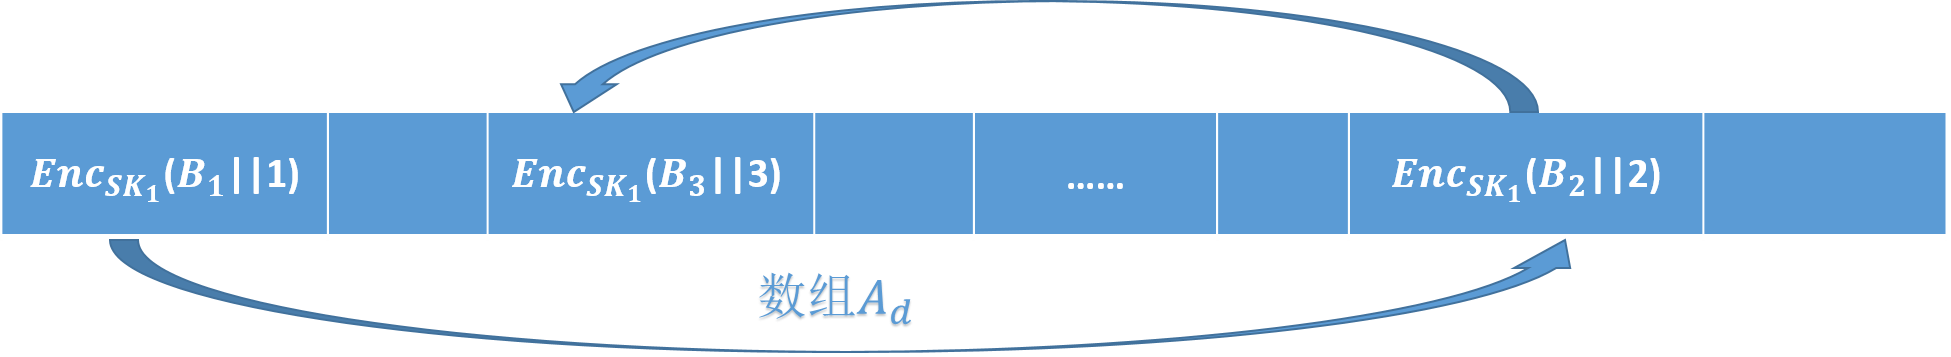
\includegraphics[width=0.95\textwidth]{chap3/file_list}

  \bicaption[fig:file_block_list]{加密后文档块链表}{加密后文档块链表} {Fig}{Document Block List of Encryption}
\end{figure}


\textbf{索引建立($BuildSIndex$)} 首先对所有文档集$D$,提取出$D$中所有不同的单词集合$W(D) = \{w_1, ..., w_{|W(D)|} \}$;然后对每个单词$w_i \in W(D)$,使用伪随机置换函数 $\pi_{K_1}$生成一个置换后的单词集合$PW = \{\pi_{K_1}(w_1), ..., \pi_{K_1}(w_{|W(D)|} \}$。

随后,我们选取$|W(D)|$个$l-2$ 维的标准化正交基(正交基的建立过程可以使用史密斯正交化理论构建
\cite{daniel1976reorthogonalization}):$\{e_1, ..., e_{|W(D)|}\}$ ,$|e_i| = l-2$,$i \in [1, |W(D)|]$;然后将每个置换后的单词与对应的正交基拼接起来,则每个单词$w_i$的结构如下:$\pi_{K_1}(w_i) || e_i$,且每个结构的大小为$l-1$ 维;再分别将集合$[1,q]$中每个数与变化后的单词结构相连接,则最终对每个单词$w_i$形成$q$个$l$ 维的空间向量,对$1 \leq i \leq |W(D)|$ 和$1 \leq j \leq q$,其结构为$f_{w_i,j} = (\pi_{K_1}(w_i) || e_i || j)$。
对每个变量$f_{w_i,j}$,使用伪随机函数$F_{K_2}$生成一个结果放入查找表(look-up)$T$中,在$T$中每个结点存储的内容如下:
\begin{center}
    $T[F_{K_2}(f_{w_i,j})] = <f_{w_i,j}, addr_{ID}(ID(w_i)[1])> \oplus \mathcal{G}(P_{K_3}(f_{w_i,j}))$,
\end{center}
这里$F_{K_2}$和$P_{K_3}$是伪随机函数,$\mathcal{G}$是伪随机生成器,$addr_{ID}(ID(w_i)[1])$是指单词$w_i$所对应的文档$ID$集合在文档$ID$数组$A$中的第一个文档ID所存放的地址。


对每个单词$w_i \in W(D)$,建立文档$ID$的集合$ID(w_i) = \{ID(D_i) | w_i \in D_i \}$,并填充是所有的集合$|W(D)|$大小相等;然后对每个$ID(w_i$建立链表$L_{w_i}$,使之在$ID(w_i)$中每个元素($1 \leq j \leq |ID(w_i)|$)在数组$A_s$ 中的结构如下:
\begin{center}
$A[addr_{ID}(ID(w_i)[j])] = (<ID(w_i)[j], addr_{ID}(ID(w_i)[j+1])> \oplus H(Q_{K_4}(f_{w_i,j}),r_i), r_i)$,
\end{center}
这里$r_i$ --- 随机字符串,$ID(w_i)[j]$ --- 表示集合$ID(w_i)$中的第$j$个元素,$addr_{ID}(ID(w_i)[j])$ --- 表示元素$ID(w_i)[j]$存放在数组$A$中的地址,$Q_{K_4}$ --- 表示伪随机函数,$H$ --- 表示伪随机置换。

如$q = 2$,对包含三个单词的文档,按照上述方式,构建完成后的安全索引结构如下图\ref{fig:resist_secure_index} 所示:
\begin{figure}[!htp]
  \centering
  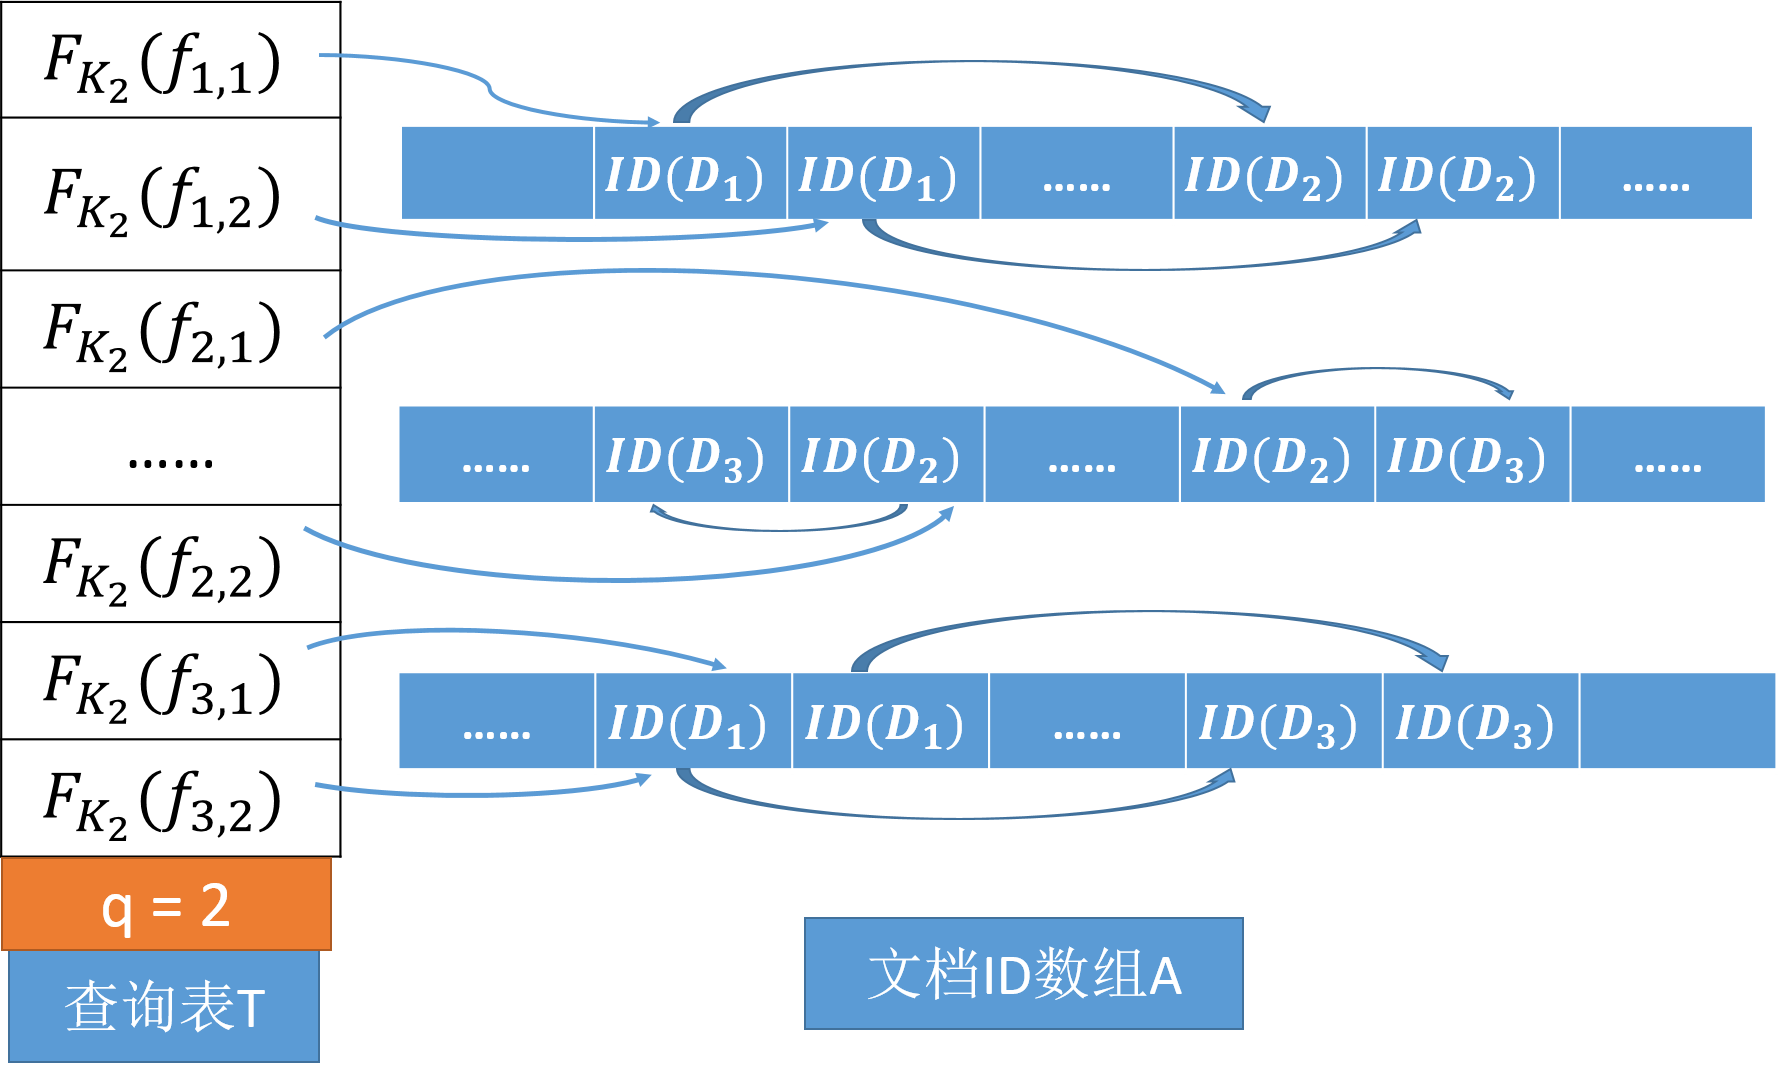
\includegraphics[width=0.95\textwidth]{chap3/resist_secure_index}

  \bicaption[fig:resist_secure_index]{抗泄漏方案的安全索引}{抗泄漏方案的安全索引} {Fig}{Secure Index of Resisting Information Leakage}
\end{figure}

数据拥有者在加密过程中主要使用了两个函数:文档加密函数$DEnc$ \ref{alg:DEnc}和安全索引建立算法$BuildSIndex$ --- 包括两个子算法:$BuildLookup$ \ref{alg:BuildLookup}与$BuildArray$ \ref{alg:BuildArray},其具体实现过程分别如下:

%%
%%  algorithm: DEnc
%%
\begin{algorithm}[!htb]
\caption{$A_d \leftarrow DEnc(D, K)$}
\label{alg:DEnc}
\begin{algorithmic} [1]

\ENSURE ~~\\
  \COMMENT{ \textbf{Initialization}} ~~\\
         allocate enough array: $A_d$ ~~\\
         make each $|D_i|$ equal by filling ~~\\
  \COMMENT{ \textbf{Build List for $D$}} ~~\\
  \STATE divide each $D_i \in D$ into m blocks:$D_i = (B_1, ..., B_m)$
  \STATE add unique location flag to $D_i$, get: $B$ =($B_1||1, ..., B_m||m$)
  \STATE make $p$ copies of $B$, and randomly shuffle for each one 
         \FOR {$1 \leq j \leq p$}
           \FOR { $B_i \in B$}
              \STATE create a node: $A_d[addr_D(B_i)] = < SKE.Enc_{SK_j}(B_i), addr_D(B[i+1]) >$,
                     where $addr_D(B_i)$ is randomly unique address. ~~\\
                     for the last block, having: $addr_D(B_m) = NULL$ ~~\\
           \ENDFOR
         \ENDFOR
  %
  % RETURN VALUE OF THE ALGORITHMS
  %
  \RETURN ${A_d}$;

\end{algorithmic}
\end{algorithm}

%%
%%  algorithm: BuildLookup
%%
\begin{algorithm}[!htb]
\caption{$T \leftarrow BuildLookup(D,K)$}
% algorithm label to be referred in the text
\label{alg:BuildLookup}
\begin{algorithmic} [1]

\ENSURE ~~\\
  \COMMENT{ \textbf{Initialization}} ~~\\
  \STATE allocate enough look-up table $T$ ~~\\
         select orthogonal basis $\{e_1, ..., e_{|W(D)|} \}$ of $l-2$ dimensions ~~\\
         randomly select constant $q$ ~~\\
  \COMMENT{ \textbf{Build Look-up Table $T$}} ~~\\
         \FOR {$w_i \in W(D)$}
           \STATE generate: $t(w_i) = \pi_{K_1}(w_i) || e_i$, $|t(w)| = l-1$
           \FOR {$1 \leq j \leq q$}
             \STATE get: $f_{w_i,j} = t(w_i) || j$ ~~\\
             \STATE for $f_{w_i,j}$, create a node: ~~\\
                    $T[F_{K_2}(f_{w_i,j})] = <f_{w_i,j}, addr_{ID}(ID(w_i)[1])> \oplus \mathcal{G}(P_{K_3}(f_{w_i,j}))$

           \ENDFOR
         \ENDFOR
         \STATE fill remaining blanks to random value.
  %
  % RETURN VALUE OF THE ALGORITHMS
  %
  \RETURN ${T}$;
\end{algorithmic}
\end{algorithm}

%%
%% algorithm: BuildArray
%%
\begin{algorithm}[!htb]
\caption{$A \leftarrow BuildArray(D,K)$}
\label{alg:BuildArray}
\begin{algorithmic} [1]

\ENSURE ~~\\
  \COMMENT{ \textbf{Initialization}} ~~\\
  \STATE get $ID(w_i)$ of $w_i \in W(D)$ ~~\\
         assure all $|ID(w_i)|$ equal ~~\\
         allocate enough array $A$ ~~\\
  \COMMENT{ \textbf{Build Array $A$}} ~~\\
         \FOR {$w_i \in W(D)$}
           \FOR {$1 \leq j \leq |ID(w_i)$}
             \STATE create a node in $A$:  \ \ $A[addr_{ID}(ID(w_i)[j])] = $ ~~\\
                    $<ID(w_i)[j], addr_{ID}(ID(w_i)[j+1])> \oplus \mathcal{H}(Q_{K_4}(f_{w_i,j},r_i), r_i)$ , ~~\\
                    and for last node: $addr_{ID}(ID(w_i)[|ID(w_i)|]) = NULL$.
           \ENDFOR
         \ENDFOR
         \STATE fill remaining entries of $A$ to random value
  %
  % RETURN VALUE OF THE ALGORITHMS
  %
  \RETURN ${A}$;

\end{algorithmic}
\end{algorithm}


\subsection{陷门生成}
\label{sec:searchpattern_trapdoor_generator}

当授权的用户使用单词$w$查询时,首先调用函数$BuildLookup$得到该单词对应的$l-1$维的向量$t(w)$,然后从集合$[1,q]$中随机选取一个数$N$,并将两者连接起来形成一个$l$维的向量$f_{w,N} = (t(w)||N)$;对向量$f_{w,N}$,构建其$l$维的法平面方程$M$ \cite{schwarzenberger1961vector},满足:
\begin{center}
$M(x_1, x_2, ..., x_l) = 0$ ($x_i$为第$i$维空间的标量值),
\end{center}
在法平面M上,我们随机选择一个与$f_{w,N}$垂直的向量$V_{f_{w,N}}$,计算其陷门$T_w$,包括:$T_w = (F_{K_2}(f_{w,N}), P_{K_3}(f_{w,N}), Q_{K_4}(f_{w,N}), V_{f{w,N}} )$,然后将陷门提交给云服务端进行搜索。具体的描述如算法 \ref{alg:TrapdrGen}。

\begin{algorithm}[!htb]
\caption{$T_w \leftarrow TrapdrGen(w,K)$}
\label{alg:TrapdrGen}
\begin{algorithmic} [1]

\ENSURE ~~\\
  \COMMENT{ \textbf{Initialization}} ~~\\
  \STATE randomly select number $N$ from set $[1,q]$ ~~\\
         get $e_i$ following algorithm $BuildSI$ ~~\\

         \COMMENT{ \textbf{Build Array $A$}} ~~\\
         \FOR {$w_i \in W(D)$}
           \FOR {$1 \leq j \leq |ID(w_i)$}
             \STATE create a node in $A$:
                    $A[ID(w_i)[j]] = <ID(w_i)[j], addr_{ID}(ID(w_i)[j+1])> \oplus \mathcal{H}(Q_{K_4}(f_{w_i,j},r_i), r_i)$ ~~\\
                    and for last node: $addr_{ID}(ID(w_i)[|ID(w_i)|]) = NULL$
           \ENDFOR
         \ENDFOR
         \STATE fill remaining entries in $A$ to random value
  %
  % RETURN VALUE OF THE ALGORITHMS
  %
  \RETURN ${A}$;
\end{algorithmic}
\end{algorithm}



\subsection{查询}
\label{sec:searchpattern_scheme_search}
%在加密阶段,所有待外包数据都已经通过加密建立安全结构并存储到云服务器上。
一旦收到授权用户发送过来的请求陷门后,云服务器将进行查询并返回结果给请求者,过程如下:
\begin{enumerate}
  \item 搜索查找表$T$:解析陷门$T_w$,在look-up中查找获得文档$ID$的入口地址;

  \item 查找数组$A$:通过文档$ID$首地址得到所有文档数据块的首地址;

  \item 查找数组$A_d$:逐个对每个文档数据块的首地址遍历直至完成,最终得到所有的文档数据块集合;

  \item 返回:将查找得到的所有结果返回给请求者。
\end{enumerate}
算法\ref{alg:Query}使用伪代码描述了Query的具体实现。

\begin{algorithm}[!htb]
\caption{$R \leftarrow Query(T_w, I, A_d)$}
\label{alg:Query}
\begin{algorithmic} [1]
\ENSURE ~~\\
  \COMMENT{ \textbf{Visit Look-up Table $T$}} ~~\\
  \STATE parse $T_w$ as: $T_w = (t_1, t_2, t_3, t_4)$ ~~\\
         set: $T[t_1] \oplus \mathcal{G}(t_2) = (a_1, a_2)$ ~~\\
  \COMMENT{ \textbf{Visit Array $A$} } ~~\\
  \IF {$a_1 . t_4 == 0$}
    \STATE init set: $ID = \varnothing $
    \STATE get: $(id, a_2) = A[a_2][1] \oplus \mathcal{H}(t_3,a[a_2][2]))$
    \STATE put $id$ into set $ID$
    \IF {$a_2 \neq NULL$}
      \STATE goto: 4
    \ENDIF
    \STATE init set: $R = \varnothing$ ~~\\
    \COMMENT{ \textbf{Visit Array $A_d$} } ~~\\
    \FOR {$1 \leq k \leq |ID|$}
      \STATE get block set: $R_k$ by traversing $ID[k]$ in $A_d$
      \STATE put $R_k$ into $R$
    \ENDFOR
  \ELSE
    \STATE exit;
  \ENDIF

  \RETURN ${R}$;
\end{algorithmic}
\end{algorithm}



\subsection{解密}
\label{sec:searchpattern_scheme_decryption}

若授权用户收到远程服务器回送的响应结果$R$后,对其进行解密,并逐步将各个数据块连接起来丢弃无用的数据块,形成完整的文档,得到用户所需求的答案$PD$。解密算法$Dec$ \ref{alg:dec}描述如下:
\begin{algorithm}[!htb]
\caption{$PD \leftarrow Dec(R, K)$}
\label{alg:dec}
\begin{algorithmic} [1]
\ENSURE ~~\\
  \STATE init: $PD = \varnothing $ ~~\\
  \COMMENT{ \textbf{Analyze each set $R_i$ in $R$}} ~~\\
  \FOR {$1 \leq i \leq |R| $}
    \STATE get corresponding $SK_N$ of $f_{w,N}$
    \FOR {$1 \leq j \leq |R[i]|$}
      \STATE decrypt: $ b_j = SKE.Dec_{SK_N}(ED[i][j])$
    \ENDFOR
    \STATE sort: $p_1, p_2, ..., p_m$ in actual block sort
    \STATE get document: $D_j = p_j[1]||p_2[1]||...||p_m[1]$
    \STATE throw dummy strings of $D_j$, put $D_j$ to $PD$
  \ENDFOR
  \RETURN ${PD}$;
\end{algorithmic}
\end{algorithm}





\section{安全性证明}
\label{sec:searchpattern_security_analysis}

基于系统模型\ref{fig:general_system_model},我们选择常用的证明模型即IND-CKA(Choosen Keyword Attatck),对查询各阶段的过程有所修改,游戏过程模拟如图\ref{fig:searchpattern_attack_model}所示。然后证明敌手在多项式时间内仅能以1/2+$negl(k)$的概率猜出游戏答案。
\begin{figure}[!htp]
  \centering
  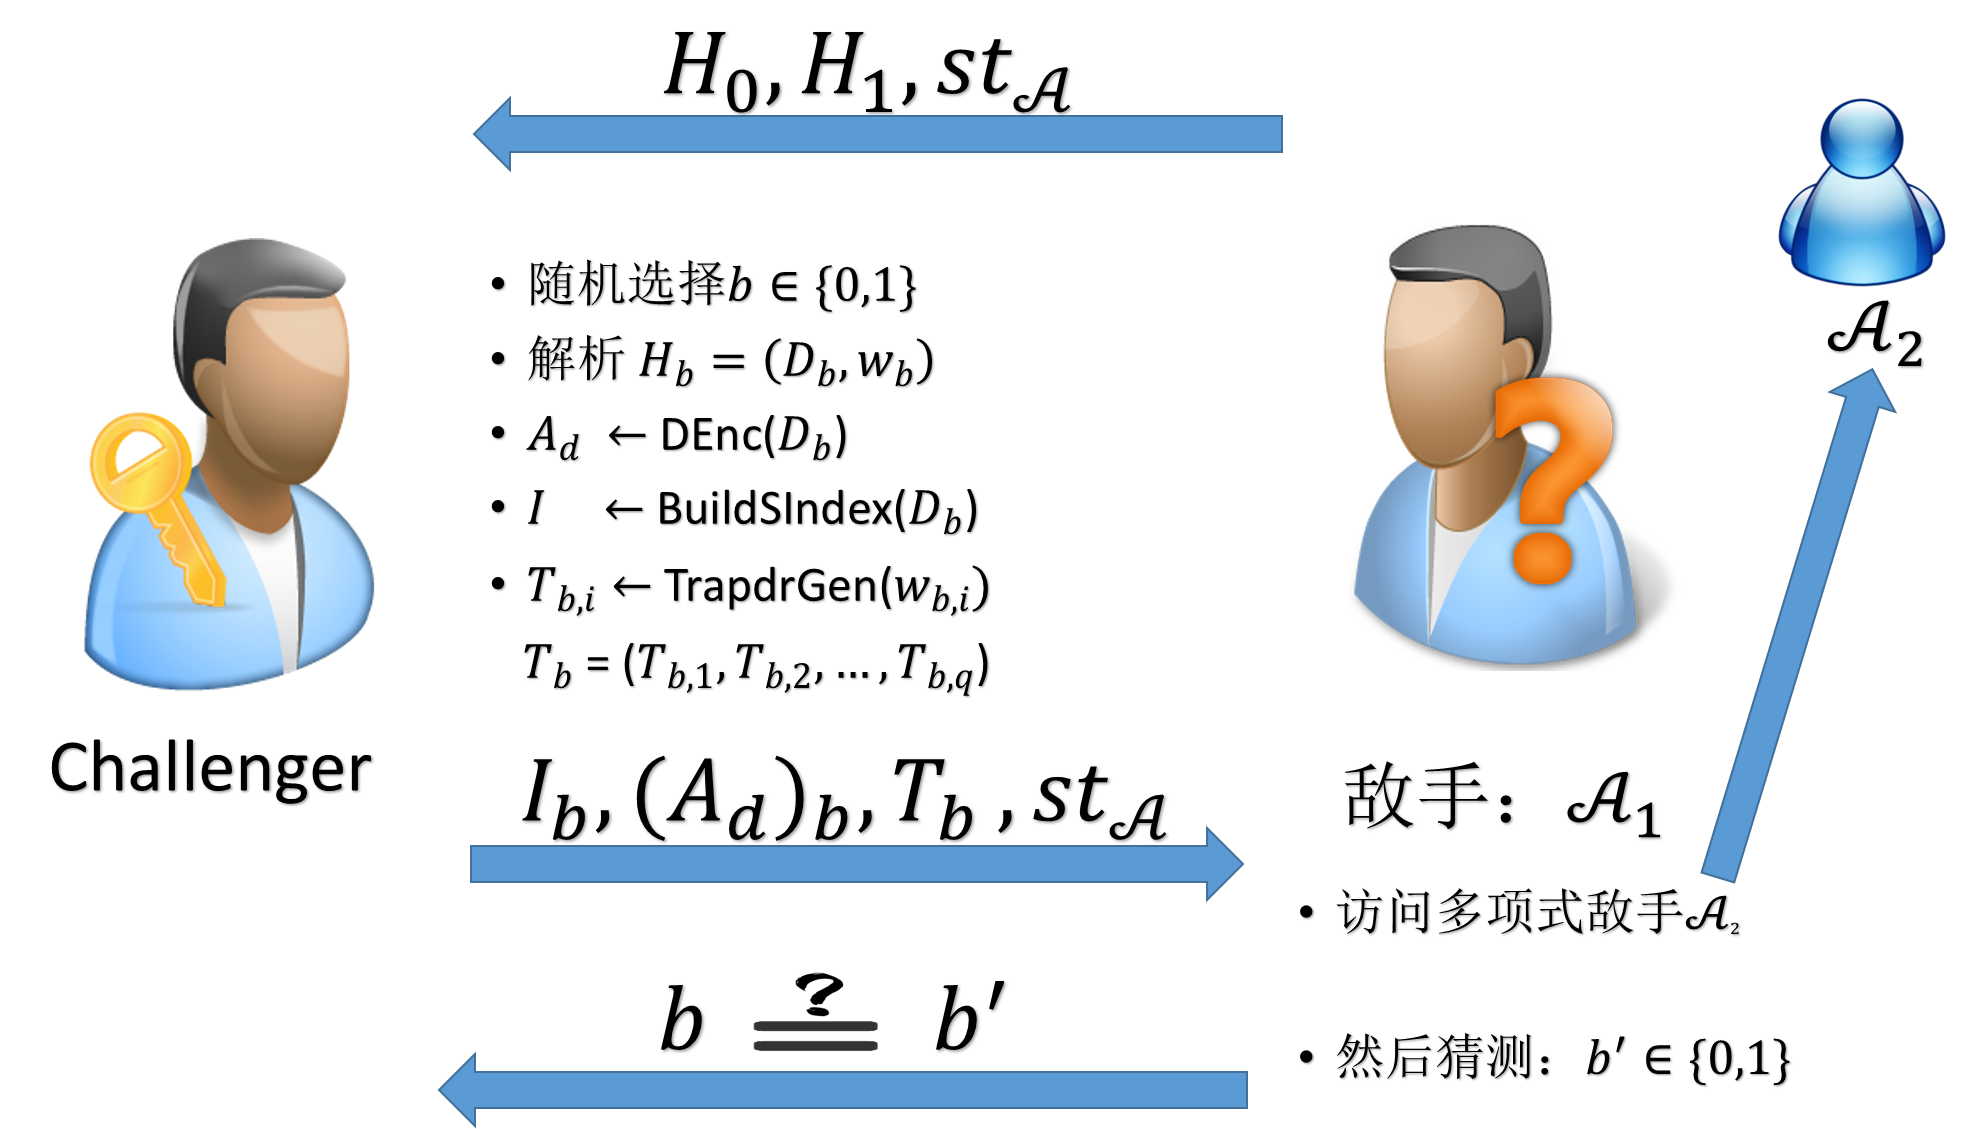
\includegraphics[width=0.9\textwidth,scale=0.8]{chap3/searchpattern_attack_model}
  \bicaption[fig:searchpattern_attack_model]{修改后的方案游戏模型}{修改后的方案游戏模型}{Fig}{New Security Game Model}
\end{figure}

\begin{thm}[$IND\_CKA$ Security]
\label{thm:ind_cka_security_proof}

如果方案中所使用的函数$F$、$P$和$Q$是伪随机函数,$H$和$\phi$是伪随机置换,$\mathcal{G}$是伪随机生成器,并且$SKE$是$PCPA$安全的,则该方案是non-adaptive不可区分安全的。

\begin{proof}
该部分将使用Curtmola方案中提出的Non-adaptive不可区分游戏模型对方案的安全性进行证明。

在游戏过程中,首先敌手$\mathcal{A}_1$发送的历史记录$H_0$和$H_1$,满足$|H_0| = |H_1|$即$|D0| = |D1|$ 且$|w0| = |w1|$, 然后挑战者(Challenger)在过程中随机选择参数b,敌手$\mathcal{A}_1$收到记录后能访问多项式敌手$\mathcal{A}_2$,但在猜测过程中,仅能使用挑战者获得的知识。因而,我们仅仅需要判断敌手对挑战者发起的内容在多项式时间不可区分,从如下几个方面分析:

\begin{itemize}
  \item \textbf{$Setup$:}挑战者$C$随机生成密钥$K$;

  \item \textbf{$DEnc$:}当$C$收到敌手$\mathcal{A}_1$发送过来的历史信息$H_0$和$H_1$后,随机选择参数$b$,然后解析历史$H_b$并对文档加密生成$(A_d)_b$,并送至敌手;

  \item \textbf{$BuildSIndex$:}同样地挑战者收到挑战的历史记录后,对$D_b$建立安全索引$I_b$;

  \item \textbf{$TrapdrGen$:}  挑战者$C$对$w_b$中每个单词,计算对应的陷门,并送至敌手$\mathcal{A}_1$。
\end{itemize}

在上述所有过程中,挑战者仅仅使用了安全的伪随机过程和$PCPA$安全的对称加密方案SKE,它们仅都在多项式时间内以不大于1/2+$negl(k)$的概率进行区分。因此,当敌手收到$C$发送过来的信息后,即使敌手$\mathcal{A}_1$ 有能力访问算法$\mathcal{A}_2$,仍不能猜中$b' = b$ 的概率大于1/2。所以,我们的方案是non-adaptive不可区分安全的。

另外,我们的方案在搜索时,一个单词对应有$q$个不同的单词陷门,并且同一个单词陷门访问文件块时有$p$ 种情况和相同文档中一块指向下一对应块的连接是随意的(每个文件块包含$p$份),故敌手能推断出搜索模式的概率仅为$q*2^p$。因不同的单词同样含有相同的文档,故能推断出搜索模式的概率小于$q*2^p$。

\end{proof}
\end{thm}



%%%%%%%%%%%%%%%%%%%%%%%%%%%%%%%%%%%%%%%%%%%%%%%%%%%%%%%%
%%
%%    性能分析
%%
%%%%%%%%%%%%%%%%%%%%%%%%%%%%%%%%%%%%%%%%%%%%%%%%%%%%%%%%
\section{性能分析}
\label{sec:searchpattern_capability}
到此,我们已经完成了整个方案的功能,不仅能避免size pattern的泄漏,以概率泄漏搜索模式和访问模式,同时也通过严格的分析证明了我们方案在我们的模型下是安全的。下面我们从三个方面对我们方案的性能进行分析 --- 存储开销、计算开销和传输开销。

\subsection{存储开销}
\label{sec:searchpattern_capability_storage}

为了减少更多的信息泄漏,方案不得不引入额外的存储开销。下面我们从两个方面分析方案的存储性能:
\begin{enumerate}
  \item \textbf{索引结构:}在方案中,我们使用查询表$T$和数组$A$来存储安全索引。在建立查询表过程\ref{alg:BuildLookup}中,对每个单词存储p份,因而$T$的存储空间大小为:$W(D) * q * |T[i]|$ ($T[i]$ --- 表示查询表中每个结点所需要的大小)。在文档ID数组的建立过程
      \ref{alg:BuildArray} 中,对每个单词$w$,存储被文档包含的ID数组,并且通过填充使每个ID数组大小保持相等,因而数组$A$的存储空间大小至少为:$W(D) * ID(w_i) * A[i]$($w_i \in W(D)$,$A[i]$ --- 表示数组每个结点所占用空间)。

  \item \textbf{文档结构:}在加密文档过程\ref{alg:DEnc}中,首先对每个文档进行填充使大小为文档的最大大小并分块,并对每块复制$p$份,因而文档块数组$A_d$的大小至少是:$|D_i| * p$。

\end{enumerate}


\subsection{计算开销}
\label{sec:searchpattern_capability_computing}

我们从客户加密、陷门生成和服务端查询三个方面对方案的计算性能进行分析。
\begin{enumerate}
  \item \textbf{加密文档:}在数据所有者外包数据之前,首先对文档进行加密,涉及到建立索引和文档加密。在文档加密阶段,客户的计算开销花费在对数据分块是调用函数SKE.Enc进行简单的加密处理,计算时间为:$|D| * m * T(SKE.Enc)$($T(SKE.Enc)$ --- 表示算法SKE.Enc加密所使用的时间)。索引建立的时间主要包括生成斯密斯正交基和建立安全索引,其计算时间开销为:$T(s) * |W(D)| + |W(D)| * q * ID(w_i)$ ($w_i \in W(D)$, $T(s)$ --- 表示生成正交基所花费的时间)。

  \item \textbf{陷门计算:}在陷门生成算法计算过程\ref{alg:TrapdrGen} 中,首先需要获得待查寻单词$w$的一个正交基(计算过程与算法BuildLookup相同),然后基于该向量构建该向量的法平面,因而客户端的计算开销为:$T(s) + T(M)$,这里$T(s)$和$T(M$分别表示生成单词$w$的基和该基向量的法平面所需要的时间。

  \item \textbf{文档查询:}在算法Query\ref{alg:Query}过程中,服务器需要分别遍历安全索引和文档块数组,这里假设在数据$A$和$A_d$中单步的计算开销为$O(1)$,则总时间计算开销为:$|ID(w_i)| * m$ ($w_i \in W(D)$,$m$ --- 表示每个单词所查找到的所有文件块总大小)。
\end{enumerate}

\subsection{传输开销}
\label{sec:searchpattern_capability_transmission}

传输开销主要发生在客户与服务器之间的通讯阶段,因而,我们可以从上传文档、发送搜索陷门和返回检索结果这三个方面来分析网络的负荷。

\begin{enumerate}
  \item \textbf{文档上传:}在文档上传阶段,客户上传至服务端的信息包括索引结构$I$ 和加密文档结构,因而该次通讯开销的总大小为:$|A| + |T| + |A_d|$。

  \item \textbf{搜索陷门提交:}在该阶段,用户上传的陷门内容仅仅包括待查单词的几个伪随机函数,因而我们可以简单地将通讯时间看作为$O(1)$,与其它方案的开销保持在同一个级别。

  \item \textbf{检索结果返回:}在服务器返回符合搜索条件的结果至客户过程中,传输的信息量记为查询过程所得的结果大小,因而传输开销的大小同样为:$ID(w_i)| * m \ (m \approx |D_i|)$ 。由于在每次用户查询过程中,都需要计算和传输该数据,因而应该尽可能地减小其大小。

\end{enumerate}





%%\section{基于可信第三方的方案}
%%\label{sec:searchpattern_trusted_third_party}
%%
%%这里,简单介绍一个如何使用可信第三方来真正确保trace信息的泄漏。使用可信第三方的系统模型如图
%%\ref{fig:searchpattern_trusted_third_party}所示:
%%\begin{figure}[!htp]
%%  \centering
%%  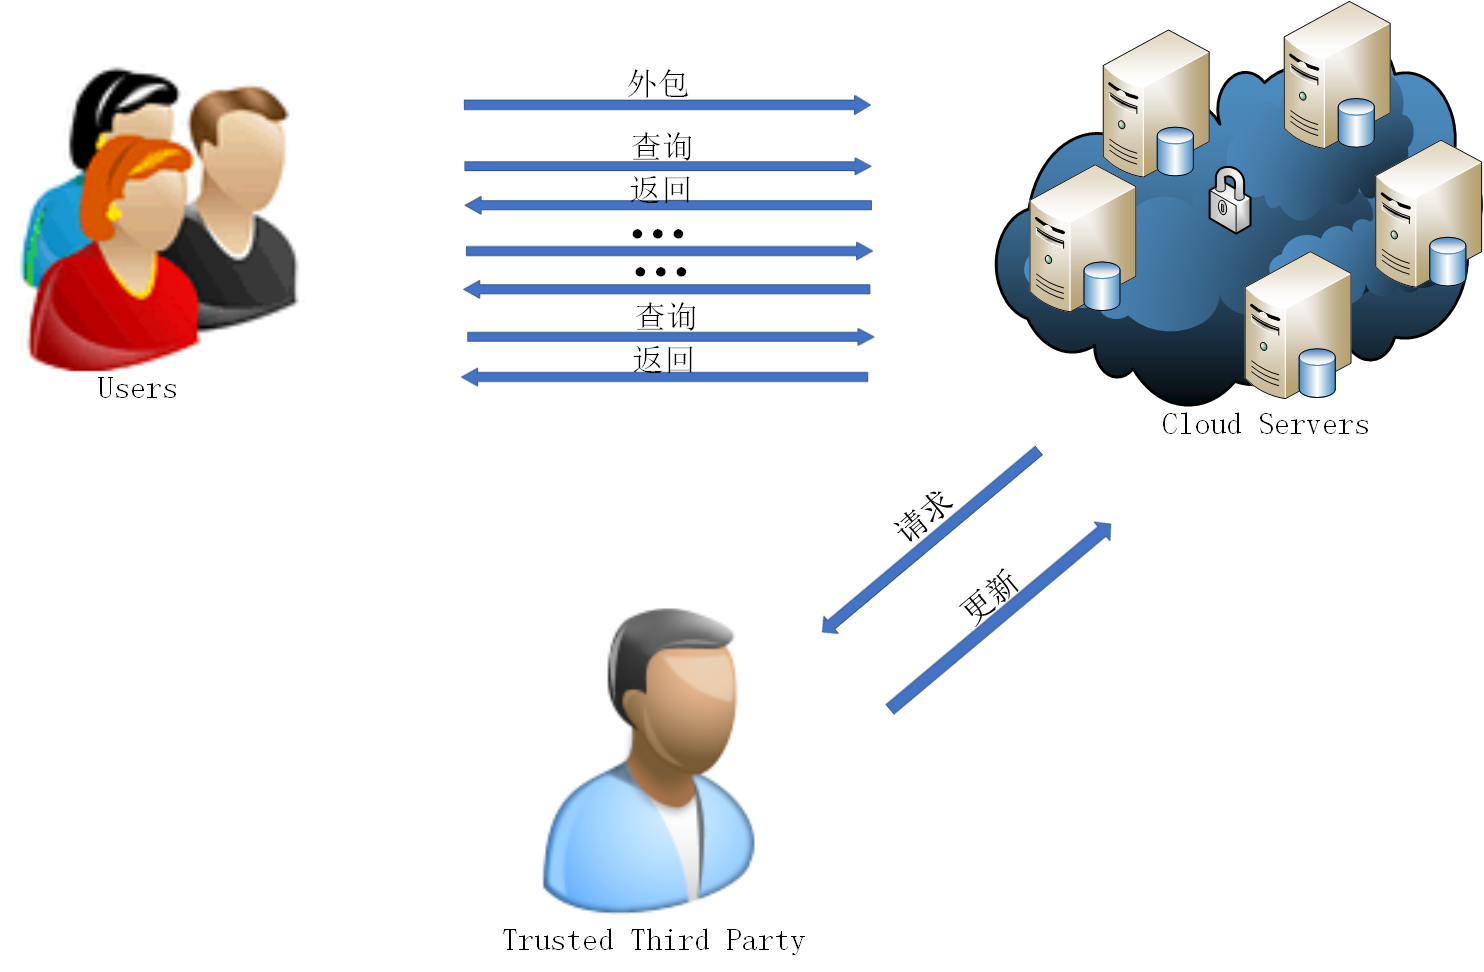
\includegraphics[width=0.9\textwidth,scale=0.8]{chap3/searchpattern_trusted_third_party}
%%  \bicaption[fig:searchpattern_trusted_third_party]{基于可信三方的系统模型}{基于可信三方的系统模型} {Fig}{The System Model Based on Trusted Third Party}
%%\end{figure}
%%
%%在该模型中,我们设计的方案与上述可搜索加密算法相比,主要在以下几个过程上有所不同:
%%\begin{itemize}
%%  \item \textbf{安全索引的存储:}由可信第三方存放安全索引;
%%
%%  \item \textbf{陷门生成:}授权用户提交陷门至可信第三方;
%%
%%  \item \textbf{结果查找:}可信第三方将所需的文档信息发给给服务器,服务器之间返回结果给请求者。
%%\end{itemize}

%%\section{基于三方方案的构造}
%%\label{sec:searchpattern_how_build}

%%\section{应用}
%%\label{sec:searchpattern_application}


